\chapter{Eredmények}
\pagestyle{headings}


\section{Sejtekből kiszabaduló káliumion koncentráció közelítő számítása}
A kísérletes munkát megelőzően számolásokat végeztem el annak érdekében, hogy felderítsem azt, hogy az elektród egyáltalán képes lehet-e detektálni az összes sejt szétesést követően az extracelluláris tére felszabaduló kálium-ion koncentrációját. Hiszen mint minden mérőszközzel, így a kálium- ionszelektív elektróddal is csak meghatározott tartományon belül lehet pontos mérést végezni. A tipikus ionszelektív elektród alsó kimutatási határa 10$^{-6}$, 10$^{-6}$ M. 
 A számolás lépései a következőek voltak. Megnéztem az általam vizsgálandó fajra (\emph{Candida albicans}) jellemző sejttérfogatot \cite{chaffin1984relationship}, ami körülbelül (ide kéne érték) $\upmu m^3$/. Kiszámoltam, hogy 10 cm$^3$  oldatban mennyi a teljes intracelluláris térfogat, ha a sejtszám 1 cm$^3$ térfogatban 10$^7$ db sejt. Az intracelluláris kálium-ionkoncentráció (0.1 M, hivatkozás kell ide is) és a teljes intracelluláris térfogat(2 $\cdot$ 10$^9$ $\upmu m^3$) szorzatából kiszámoltam 2 $\cdot$ 10$^{-6}$ $dm^3$ sejttérfogatban lévő teljes kálium-ion anyagmennyiséget (2 $\cdot$ 10$^{-7}$ mol), majd ezt elosztottam az oldat (0.01 $dm^3$) térfogatával, így megkaptam a teljes extracelluláris kálium-ionkoncentrációt (2 $\cdot$ 10$^{-5}$ M) arra vonatkozóan, ha az összes sejt károsodást szenvedne. A kapott eredmények alapján elmondható, hogy elvégezhető a mérés, mert a számolt kálium-ionkoncentráció nagyobb, mint a legkisebb koncentráció, amit az elektród még képes detektálni/kimutatni. 

\section{Káliumion szelektív elektródok kalibrációja}
A méréshez használt elektródokon kalibrációt végeztem el, hogy a kapott egyenes egyenletének segítségével a potenciálértékekből tudjak koncentrációt számolni. A jobb nyomonkövethetőség és érthetőség érdekében bizonyos lépéseket újból leírok. Az elektródokat úgy kalibráltam, hogy a töményebbtől a hígabb oldat felé haladva belemerítettem az elektródot és t = 1 min időpontban mért potenciált jegyeztem fel. A kapott feszültségértékeket a káliumion- koncentráció tízes alapú negatív logaritmusának függvényében ábrázoltam, majd megszerkesztettem a kalibrációs egyenest lineáris regresszióval, hogy megkaptam az egyenes egyenletét. Ezeket a lépéseket mindhárom elektród esetében elvégeztem.

A kalibrációs egyenesek és a kiszámolt szelektivitási együtthatók alapján elmondható, hogy zavaró ionok közül a legkevésbé zavaró hatást a nátrium ionok jelentik, mert a hidrogén és az ammóniumion kisebb koncentrációja esetén nagyobb a szelektivitási együttható értéke, mint a nátriumion esetén (ide azért kéne számérték. vagy a szelektivitás, vagy az összehasonlító adat, ami a kis füzetben meg volt adva).  Az egyenes meredeksége megadja, hogy ha az oldat tízszeresére hígul vagy töményedik, akkor mennyi lesz (az egységnyi koncentrációváltozás esetében: nem egységyni, az előbb írtad le, hogy tízszeres) a bekövetkező potenciálváltozás, ez az általam használt elektródok esetén 54.76-53.188 mV/dekád között változott, ami megközelíti a kézikönyvben közölt adatot (elektródonként le kell írni az egyenes egyenletét, és utalni kell az ábrára, amit mellesleg el kéne készítened, és feltölteni a dokumentum mellé).

ez a rész már a következő "section"-be való, hiszen ez már nem kalibráció, hanem a mérés:
 A mérés kezdetén a kezeletlen szuszpenziókba merült mindhárom elektród. Mindhárom elektród esetében nem változott a potenciál, viszont mikor adott időpontban hozzá az egyik szuszpenzióhoz a nysztatint, a másik szuszpenzióhoz a propoliszt és a harmadikat pedig kezeletlenül hagytam (ez a mondat nagyon sántít). Meglepően gyorsan fejtette ki hatását a nysztatin, ami a potenciálváltozásban is szemmel látható volt, mert a görbe meredeken emelkedett egészen az egyensúly beálltáig. Ezzel szemben a propolisszal kezelt szuszpenzióban kevésbé volt meredek a detektált változás, a kezeletlen szuszpenzióban. Nagyjából tízszeres változás figyelhető meg a két pozitív kontrol potenciálváltozása között, ami a kiáramlott káliumion-koncentrációváltozásban is megmutatkozik. 

\section{Káliumion kiáramlás nyomon követése ionszelektív elektróddal}
Ha ezt a kísérletet valamely mintavételi módszerrel végeztem volna el, akkor csak a kiindulási állapotot (amikor még nem adtam hozzá egyik befolyásoló szert sem a szuszpenzióhoz) és a végállapotot (mikor a nysztatin változást okoz, és a sejtfalat roncsolja, így hirtelen nagy mennyiségű káliumion kiáramlik) tudtam volna csak vizsgálni és csak a változás lett volna detektálható. Viszont in situ online módszert alkalmazva detektálható volt a roncsolás időtartama és az ezt követő időszak is, mikor a teljes káliumion mennyiség kiáramlott az extracelluláris. 

A propolis görbéjéről (nem a propolis görbéje, ponotsabban fogalmazz) azt lehet leolvasni, hogy ha dezorganizáló hatású anyagot juttatunk a szuszpenzióba, akkor a sejtpusztulás és a káliumion kiáramlás folyamata hosszabb időt vesz igénybe, míg végül eléri ugyanazt a végkoncentrációt, mint amit a nysztatin esetén tapasztaltam, ahol pillanatok alatt (pontos adat: mennyi idő) lezajlott a sejtfal roncsolódása és a káliumion extracelluláris térbe történő kiáramlása. A negatív kontrol mintában egészen addig nem volt tapasztalható változás, ameddig hozzá nem adtam a nysztatint. 


ide azért részletesebb leírás kell. ezt sokszor megbeszéltük. sokkal több következtetés van. a nisztatinos és oldószeres kontrollról nem írtál. fontos, hogy azokra nem reagált az elektród. mit jelent ez: a tapasztalt potenciálváltozást csak a káliumion koncentráció változás okozhatta, hiszen minden más változót megvizsgáltál - ami változik a mérés során - és egyik esetben sem tapasztaltál potenciálváltozást.

mi volt a lényege a mérésnek biológiai szempontból? a propolis köztudottan antifungális szer, de nem tudni pontosan, hogyan fejti ki a hatását. te kiderítetted, hogy a hatás egyik eleme az, hogy roncsolja a sejtfalat, de kevésbé mint pl. a nisztatin, ami azonnal, néhány perc alatt az összes sejtet szétroncsolja. A mérési görbéről (xy. ábra, kék jelölésű görbe) egyértelműen leolvasható, hogy lassú, de határozott káliumion koncentráció növekedés volt a propolis hozzáadást követően. Honnan tudjuk, hogy ezt a propolis okozta és nem roncsolódott volna a sejtfal amúgy is? Onnan, hogy a kontroll is elvégezted, ugyanúgy jártál el ezzel, csak ehhez nem adtál semmit, tehát itt a két oldat sorsa elvált, és látjuk, hogy ha nem raktál volna semmit a propolisszal kezelt mintához, nem történt volna semmi. Mire volt való a pozitív kontroll? ...


%10$^7$ db sejt/cm$^3$ $\cdot$ 10 cm$^3$ = 10$^8$ db sejt
%10$^8$ db sejt $\cdot$ 20 $\upmu m^3$/sejt = 2 $\cdot$ 10$^9$ $\upmu m^3$ = 2 $\cdot$ 10$^{-6}$ $dm^3$
%ha az összes sejt szétesik, és az összes intracelluláris káliumion kiszabadul az extracelluláris térbe:
%2 $\cdot$ 10$^{-6}$ $dm^3$ $\cdot$ 0.1 M = 2 $\cdot$ 10$^{-7}$ mol
%2 $\cdot$ 10$^{-7}$ mol / 0.01 $dm^3$ = 2 $\cdot$ 10$^{-5}$ M


\begin{figure}
\centering
\includegraphics[width=0.7\textwidth, angle=-90]{img/meres.eps}
\caption{képaláírás}
\label{fig:mérések}
\end{figure}

Ahogy az a \ref{fig:mérések}. ábrán látható.


